\documentclass{article}

\usepackage{graphicx}
\usepackage[margin=2cm,a4paper]{geometry}
\usepackage{tcolorbox}
\tcbuselibrary{listings,skins}
\usepackage{microtype}
\usepackage[htt]{hyphenat}
\usepackage{placeins}
\usepackage{parskip}
\usepackage{listings}
\lstset{
  language=bash,
  basicstyle=\small\ttfamily,
  columns=flexible,
  breaklines=true,
  showstringspaces=false,
  frame=single
}

\begin{document}

\title{Building IaaS infrastructures on the AWS Cloud}
\author{Saul Pierotti}
\date{\today}

\maketitle

\section{Creation of an HTCondor Cluster for the Alignment of NGS Reads}
The demonstrative IaaS infrastructure described in this project consists of an HTCondor cluster of three nodes.
One node is configured as Master Node, while two nodes are configured as Worker Nodes.
The infrastructure can be easily expanded by replicating the Worker Node instances.
The Master Node was not used also as a Worker Node since the performance benefits and cost savings would be marginal.
This was done also to avoid overloading the Master Node, on which the entire cluster depends.
A shared storage space directly attached to the Master Node but available to all the Worker Nodes was also implemented using the distributed file system NFS (Sun Microsystems, 1984).

\subsection{Initialization of the Instances on the AWS Cloud}
The cloud service provider Amazon Web Services (AWS, \texttt{https://aws.amazon.com/}) was used for this project.
Worker Nodes and the Master Node were both built on similar machines.
For the Master Node, the \texttt{t2.medium} instance type was used with a 50 Gb SSD as root storage.
For the Worker Nodes, the \texttt{t2.large} instance type was used with a 50 Gb SSD as root storage.
The operating system chosen for both machine types is Ubuntu Server 18.04.4 LTS.
The Master Node and the Worker Nodes were all instantiated in the same availability zone (\texttt{us-east-1a}) so that they would be able to communicate through private IPv4 addresses.
The security group for the instances was configured as follows:

\begin{figure}[!h]
    \center
    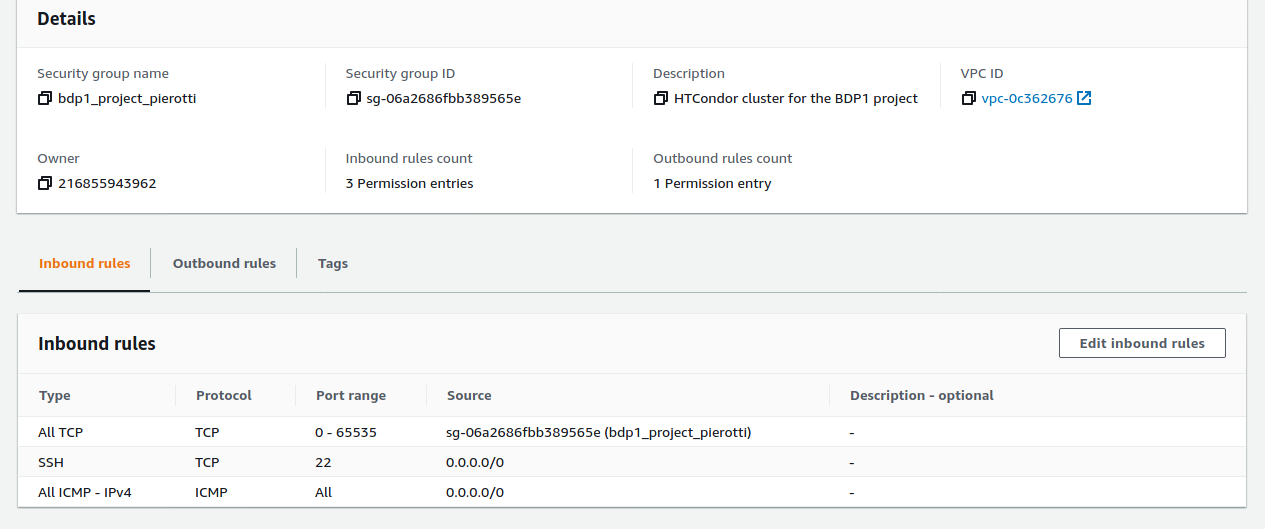
\includegraphics[width=\textwidth]{./images/security-group.png}
\end{figure}

All the TCP ports were opened to the other members of the same security group since HTCondor daemons use a dynamically assigned port.
The TCP ports were also needed for the setup of a shared NFS volume.
ICMP ports were opened for accepting incoming \texttt{ping} requests for testing purposes.
TCP port 22 was opened for allowing remote control of the machines via \texttt{ssh}.

\subsection{Configuration of the Master Node}
The PS1 prompt of the Master Node was changed so to make the node easily identifiable from the command line.

\begin{figure}[!h]
    \center
    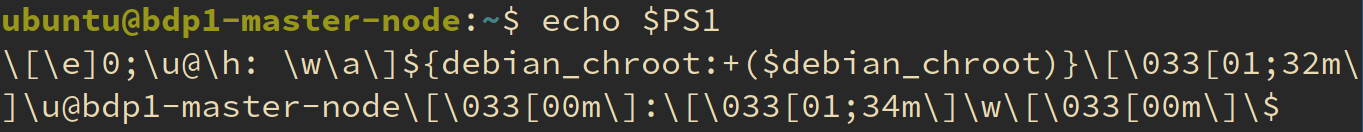
\includegraphics[width=\textwidth]{./images/master-ps1.png}
\end{figure}

HTCondor (Thain D., Tannenbaum T., and Livny M., 2005) was then installed with the following commands:

\begin{lstlisting}
sudo su
wget -qO - https://research.cs.wisc.edu/htcondor/ubuntu/HTCondor-Release.gpg.key | apt-key add - # import the gpg key of HTCondor
echo "deb http://research.cs.wisc.edu/htcondor/ubuntu/8.8/bionic bionic contrib" >> /etc/apt/sources.list # add the repository
echo "deb-src http://research.cs.wisc.edu/htcondor/ubuntu/8.8/bionic bionic contrib" >> /etc/apt/sources.list
apt update
apt install htcondor
systemctl start condor # start and enable the condor service
systemctl enable condor
\end{lstlisting}

The correct proceeding of the installation and the start of the \texttt{condor} service where checked with the following commands:

\begin{figure}[!h]
    \center
    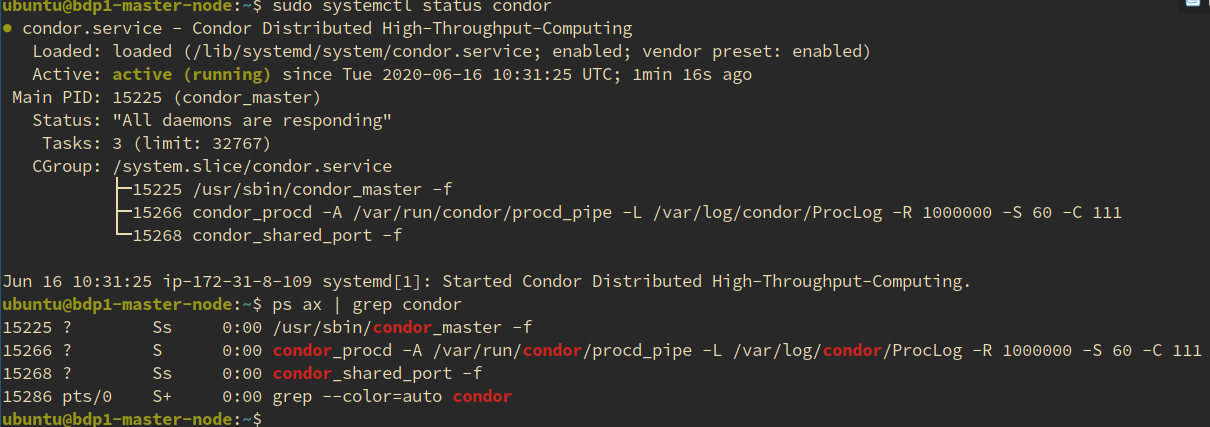
\includegraphics[width=\textwidth]{./images/condor_installed.png}
\end{figure}

The following lines where appended at the end of the main HTCondor configuration file, located at\\
\texttt{/etc/condor/condor\_config}:

\begin{lstlisting}
# Master Node IP
CONDOR_HOST = <Master_Node_private_IP>

# Master Node config 
DAEMON_LIST = COLLECTOR, MASTER, NEGOTIATOR, STARTD
\end{lstlisting}

Finally, the \texttt{condor} service was restarted with the following command:

\begin{lstlisting}
sudo systemctl restart condor
\end{lstlisting}

The NFS server was then implemented in the Master Node.
A new 100 Gb standard magnetic volume was created from the AWS interface and attached to the Master Node.
From the server, a primary partiton was initialized on the volume using \texttt{fdisk} and an \texttt{Ext4} file system was created onto it using \texttt{mkfs.ext4}.
The file \texttt{/etc/fstab} of the Master Node was modified so that the machine would mount the volume automatically at boot under the newly created directory \texttt{/data}.
The following line was appended to \texttt{/etc/fstab}:

\begin{lstlisting}
</new_volume/partiton>              /data    ext4   defaults                0 0
\end{lstlisting}

The following commands were then issued, so to install the appropriate packages:

\begin{lstlisting}
sudo apt install nfs-kernel-server
\end{lstlisting}

The following line was appended to the NFS configuration file \texttt{/etc/exports}:

\begin{lstlisting}
/data 172.31.0.0/16(rw,sync,no_wdelay)
\end{lstlisting}

Finally, the owner and group of the shared folder were changed to \texttt{nobody:nogroup} and the permissions of the folder were edited so to grant unlimited access to it:

\begin{lstlisting}
sudo chown nobody:nogroup /data
sudo chmod 777 /data
\end{lstlisting}

The \texttt{/data} folder was so made available to all the Worker Nodes on the address range \texttt{172.31.0.0/16}.
This configuration does not pose a security risk since the Master Node and Worker Nodes machines belong to a Virtual Private Cloud (VPC), and so only machines instantiated on it will be able to access the volume.
Moreover, this configuration grants immediate access to the volume to newly instantiated Worker Nodes.
A mock file was created on the \texttt{/data} folder so to be able to recognize it when mounted.

\begin{lstlisting}
touch /data/this_is_a_shared_NFS_volume
\end{lstlisting}

\subsection{Configuration of the Worker Nodes}
A virtual machine identical to the one used for the Master Node was instantiated.
The PS1 prompt of this first Worker Node was changed so to make the node easily identifiable from the command line.

\begin{figure}[!h]
    \center
    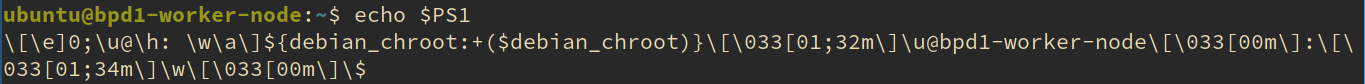
\includegraphics[width=\textwidth]{./images/worker-ps1.png}
\end{figure}

HTCondor was installed in this system with the same procedure used for the Master Node.
Only the \texttt{/etc/condor/condor\_config} file was configured differently, by appending the following lines to it:

\begin{lstlisting}
# Master Node IP
CONDOR_HOST = <Master_Node_private_IP>

# Worker Node config
DAEMON_LIST = MASTER, STARTD

HOSTALLOW_READ = *
HOSTALLOW_WRITE = *
HOSTALLOW_ADMINISTRATOR = *
\end{lstlisting}

On the Worker Node access to the shared NFS volume was then set up.
The following command was issued to install the required packages and enable the respective services:

\begin{lstlisting}
sudo apt install nfs-common
sudo systemctl start nfs-server
sudo systemctl enable nfs-server
\end{lstlisting}

A new directory was then created at \texttt{/data} using the \texttt{mkdir} command.
The \texttt{/etc/fstab} file was edited by appending the following line, so that the shared volume would be automatically mounted at boot under the directory \texttt{/data}:

\begin{lstlisting}
<Master_Node_private_IP>:/data      /data    nfs    defaults                0 0
\end{lstlisting}

It was then verified that the shared volume was accessible from the Worker Node.

\begin{figure}[!h]
    \center
    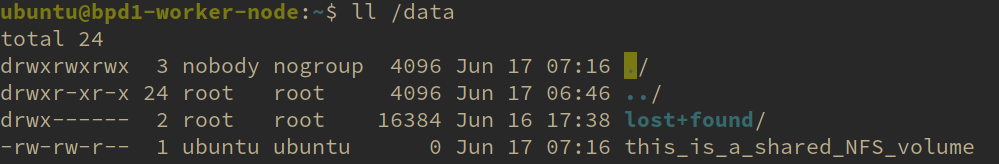
\includegraphics[width=\textwidth]{./images/nfs_works.png}
\end{figure}

On the Worker Nodes the application BWA was installed with the command:

\begin{lstlisting}
sudo apt install -y bwa
\end{lstlisting}

An image of the virtual machine was taken through the AWS interface.
In this way, the Worker Nodes would be easily replicable when more computational power is needed by instantiating new virtual machines from the image, without the need for manual configuration.

\subsection{Submission of a Test Job to the HTCondor Cluster}
For demonstrating the use of the newly created cluster, a new Worker Node was instantiated from the Worker Node image, so that the cluster would contain the Master Node and 2 Worker Nodes.

Subsequently, a new volume was created in the AWS interface from a snapshot containing test data used for the BDP1 course (\texttt{snap-09ee52d8038fb8094}, BDP1\_2020).
This snapshot contains NGS reads from 3 different patients.
Each patient has a folder with around 500 fasta files, with 1000 reads each.
Part of this data will be used for testing the infrastructure.
The new volume was mounted on the Master Node under \texttt{/data}, substituting the empty volume used before.
The \texttt{/etc/fstab} file was updated accordingly and the \texttt{nfs-server} service restarted.
It was then tested that the new volume was accessible from the Worker Nodes.

\begin{figure}[!h]
    \center
    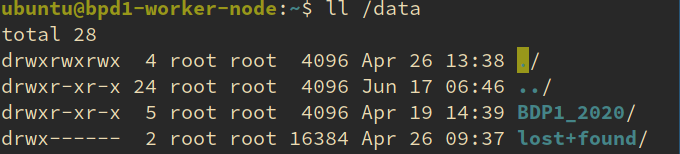
\includegraphics[width=.8\textwidth]{./images/nfs_bdp_works.png}
\end{figure}

The test job consisted in aligning ten fasta files (\texttt{read\_1.fa} to \texttt{read\_10.fa} from patient 1) to the human genome build hg19, also stored on the shared volume.
The BWA alignment tool (Li H. and Durbin R. 2009) was used for the scope.
This tool takes advantage of indexing the genome for speeding up the alignment of low-divergent reads.
The index for the hg19 build was already present in the volume snapshot, so there was no need to create it from scratch.
The test fasta files were copied from the shared volume to the home folder of the Master Node.
The test job file \texttt{alignment\_test.job} was created, with the following content:

\begin{lstlisting}
####################################################
################### Alignment Test #################
####################################################


########### The program that will be executed #######

Executable = alignment_test.py
readnum = $(Process)+1
arguments = read_$INT(readnum).fa

############ Input Sandbox  #########################

Input      = read_$INT(readnum).fa
transfer_input_files = read_$INT(readnum).fa

###### Output Sandbox ###############################

Log        = read_$INT(readnum).log
# will contain condor log

Output     = read_$INT(readnum).out
# will contain the standard output

Error      = read_$INT(readnum).error
# will contain the standard error

############## condor control variables #############

should_transfer_files = YES
when_to_transfer_output = ON_EXIT

Universe = vanilla

#####################################################

Queue 10
\end{lstlisting}

The script \texttt{alignment\_test.py} called as executable in \texttt{alignment\_test.job} was the following:

\begin{lstlisting}
#!/usr/bin/python
import sys,os
from timeit import default_timer as timer

start = timer()
dbpath = "/data/BDP1_2020/hg19/"
dbname = "hg19bwaidx"
queryname = sys.argv[1]
out_name = queryname[:-3]
fafile = queryname
samfile = out_name + ".sam"
gzipfile = out_name + ".sam.gz"
saifile = out_name + ".sai"
md5file = out_name + ".md5"

print "Input: ", queryname

command = "bwa aln -t 1 " + dbpath + dbname + " " + fafile + " > " + saifile
print "launching command: " , command
os.system(command)

command = "bwa samse -n 10 " + dbpath + dbname + " " + saifile + " " + fafile + " > " + samfile
print "launching command: " , command
os.system(command)

# Checksums
print "Creating md5sums"
os.system("md5sum " + samfile + " > " + md5file)

print "gzipping out text file"
command = "gzip " + samfile
print "launching command: " , command
os.system(command)

# Transfer files to shared volume and clean the Output Sandbox
print "Moving files and clearing the Output Sandbox"
os.system("mv "+ gzipfile + " /data/outputs/"+ gzipfile)
os.system("mv "+ md5file + " /data/outputs/"+ md5file)
os.system("rm "+ saifile)

execution_time = timer() - start

print "Total execution time: " + str(execution_time)
print "exiting"

exit(0)
\end{lstlisting}

Ten instances of this test job were run on the cluster.
The following outputs of \texttt{condor\_q} and \texttt{condor\_status} were recorded after submission:

\begin{figure}[!h]
    \center
    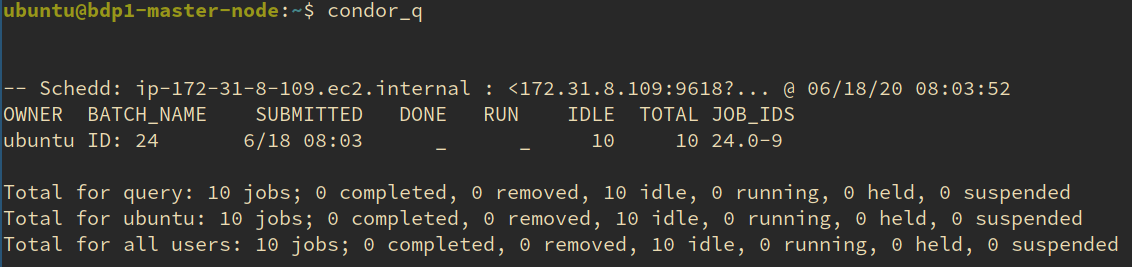
\includegraphics[width=\textwidth]{./images/condor_q.png}
    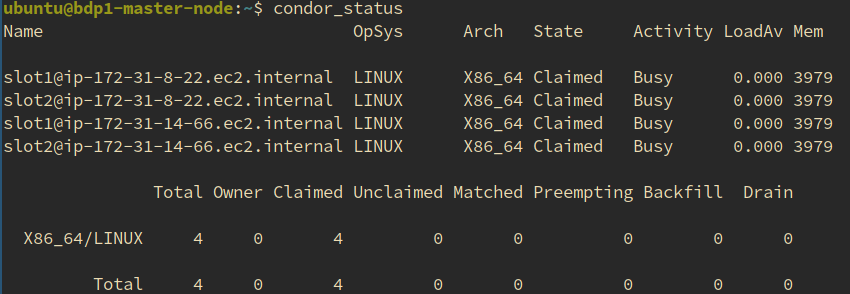
\includegraphics[width=\textwidth]{./images/condor_status_busy.png}
\end{figure}
\FloatBarrier

The cluster was able to successfully complete the task and the following output files were produced:

\begin{figure}[!h]
    \center
    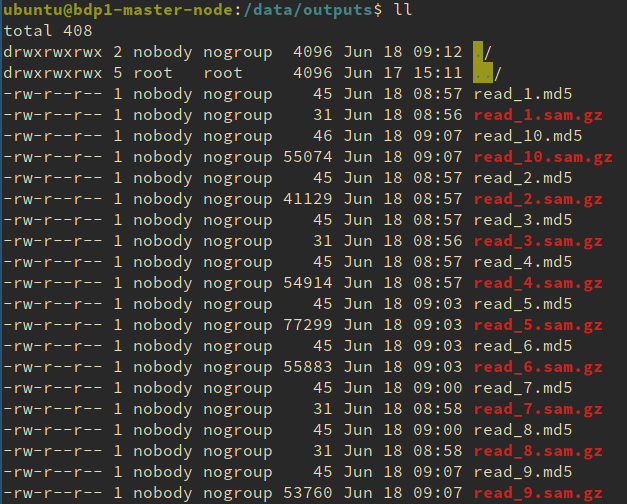
\includegraphics[width=\textwidth]{./images/condor_test_out.png}
\end{figure}
\FloatBarrier

The time required to complete the task on a single fasta file ranged from 62.77 to 422.54 seconds, with an average required time of 227.7 seconds.

\begin{figure}[!h]
    \center
    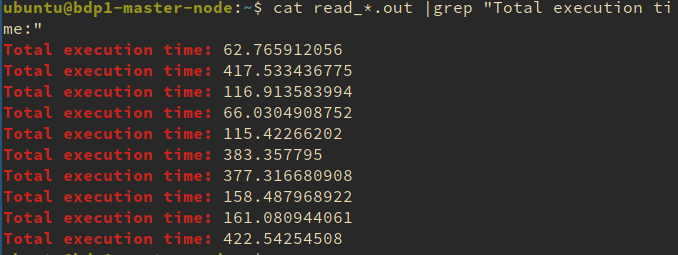
\includegraphics[width=\textwidth]{./images/time_condor.png}
\end{figure}
\FloatBarrier

\subsection{Data Management Model}
The general data management model followed is that of transferring the executables and the input fasta files using the HTCondor Input Sandbox.
This is because those files are generally small and their transfer will not overload the Master Node.
Moreover, input data are likely to be uploaded dynamically when new sequencing experiments are performed.
This system will allow sending easily new inputs to the cluster.
On the contrary, the large hg19 genome and index files will be made available to the Worker Nodes through the shared NFS volume.
The Output Sandbox will contain the condor log, the standard output, and the standard error.
These files are really small and need to be immediately available to the submitter for inspecting the proceeding of the job.
The aligned reads will instead be compressed and put in the shared volume, to avoid moving large data on the Output Sandbox.

\section{Creation of a Container Image for the Alignment of Next-Generation Sequencing reads}
A containerized version of the BWA application was built using \texttt{docker} (\texttt{https://www.docker.com/}).
A container image for the BWA application is already available on DockerHub (\texttt{biocontainers/bwa}), but for educational purposes, a new image was built from scratch.
The Ubuntu docker image was used as a base.
The local docker image \texttt{bwa} was built from the following \texttt{Dockerfile}:

\begin{lstlisting}
FROM ubuntu
RUN apt update
RUN apt install -y bwa
RUN apt install -y python
COPY ./alignment_test_docker.py alignment_test_docker.py
\end{lstlisting}

The container was then run using a bind-mount for the \texttt{/data} volume and starting an interactive shell.

\begin{lstlisting}
docker run -v /data:/data -ti bwa /bin/bash
\end{lstlisting}

The script \texttt{alignment\_test.py} was slightly modified so to omit the final data movement to the shared volume, and renamed \texttt{alignment\_test\_docker.py}.
Inside the container, the following command was run so to align a sample fasta file which had been copied from the shared volume:

\begin{lstlisting}
./alignment_test_docker.py read_1.fa
\end{lstlisting}

The application ran successfully, producing the following output in 213.33 seconds (the container was run on a Ubuntu Server 18.04.4 LTS t2.large AWS virtual machine):

\begin{figure}[!h]
    \center
    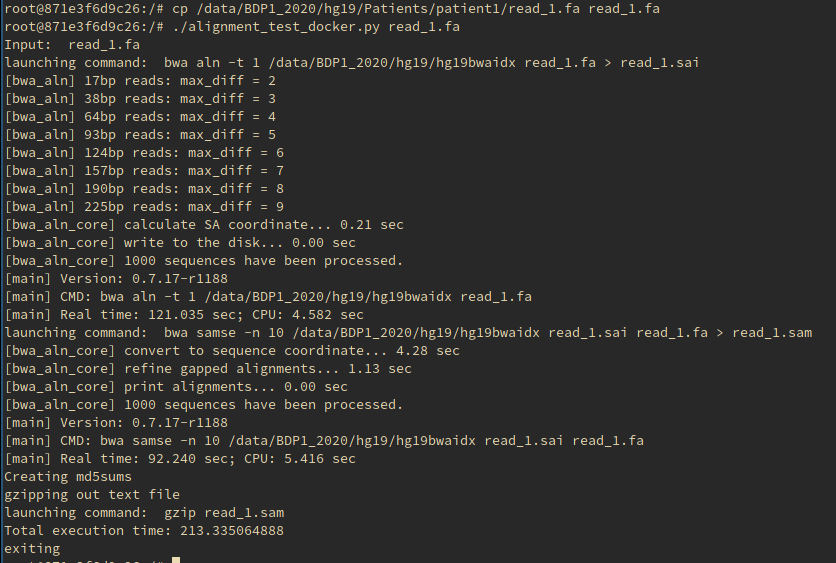
\includegraphics[width=\textwidth]{./images/docker_test_out.png}
\end{figure}

\section{Evaluation of the Resources Needed for Solving a Real Use-Case}
A plausible non-trivial use-case that can be addressed using the HTCondor cluster developed in Section 1 is the alignment of a large number of fasta files deriving from a Next-Generation Sequencing (NGS) run to the human reference genome assembly hg19.

It is recommended to aim for a coverage of at least 30x in a human Whole-Genome Sequencing (WGS) experiment (\texttt{https://www.illumina.com/science/technology/next-generation-sequencing/plan-experiments/coverage.html}).
Given that the human genome has a size of about 3.3 billion base pairs, this will result in a raw output from the sequencer of at least 99 billion base pairs.
To be on the safe side, I will consider a raw output of at least 100 billion base pairs per patient in the following cost estimate.
A single NGS read of an Illumina MySeq sequencer can have a length of up to 300 base pairs (\texttt{https://www.illumina.com/systems/sequencing-platforms/miseq.html}). Here I will consider a read length of 150 base pairs, which is recommended for a WGS experiment (\texttt{https://www.illumina.com/science/technology/next-generation-sequencing/plan-experiments/read-length.html}).
Under these assumptions, almost 667 million reads for a single patient would need to be aligned.
This amounts to about 667000 fasta files of 1000 reads each.

I roughly determined the time needed for aligning a fasta file containing 1000 reads of 150 base pairs each to the hg19 genome assembly in Section 1.
This amounts to 227.3 seconds on a single core of the AWS \texttt{t2.large} machine.
Completing the alignment of the output of a single WGS experiment would require thus 151609100 seconds of CPU time on a single core.

The cluster described in this project consists of one Master Node and two Worker Nodes.
The Worker Nodes have two cores each, so the cluster can employ a total of four cores.
In this scenario, completing the task would require 37902275 seconds, which corresponds to 1 year 2 months, and 11 days.
Of course, this running time is not acceptable.

A more feasible approach would involve replicating the Worker Nodes to have more computational power.
This is possible since the alignment of a read is completely independent from the alignment of other reads, and so the task can be run in parallel.
For instance, using a cluster of 1 Master Node and 100 Worker Nodes the task could be completed in less than 9 days.
This will result in a cluster with a capacity of 3 patients per month.

Follows a breakdown of the expected costs for aligning the output of 3 WGS experiments per month using the AWS EC2 system with On-Demand pricing on the US East N. Virginia availability zone, on a Linux system (\texttt{https://aws.amazon.com/pricing}).
To date (May 2020) the \texttt{t2.large} machine costs \$ 0.0928 per hour, and the cluster will require 100 of them for the Worker Nodes.
The \texttt{t2.medium} machine costs \$ 0.0464 per hour, and the cluster will require just 1 of them for the Master Node.
With an expected time needed for the task of 9 days, the costs for the computation for one patient will amount to \$ 1963.
Storage on general-purpose SSD EBS devices costs \$ 0.1 per Gb per month.
A 1 Tb disk can be used for storing the hg19 genome and index, as well as the reads of the patients.
Therefore, storage will have a cost of \$ 100 per month.
The total monthly cost will amount to \$ 5991.
Costs for data movements in and out of the AWS system have been omitted.
In a real use-case scenario, a strict security policy for dealing with medical data should be also enforced, according to local regulations.
This will likely increase the costs and the overhead required.

\section{References}
Li H. and Durbin R. (2009) Fast and accurate short read alignment with Burrows-Wheeler Transform. Bioinformatics, 25:1754-60. [PMID: 19451168]\\

Douglas Thain, Todd Tannenbaum, and Miron Livny, "Distributed Computing in Practice: The Condor Experience" Concurrency and Computation: Practice and Experience, Vol. 17, No. 2-4, pages 323-356, February-April, 2005.\\

Docker:\\
\texttt{https://www.docker.com/}

Recommended coverage for a WGS experiment:\\
\texttt{https://www.illumina.com/science/technology/next-generation-sequencing/plan-experiments/coverage.html}

Read lenght for a WGS experiment:\\
\texttt{https://www.illumina.com/science/technology/next-generation-sequencing/plan-experiments/read-length.html}\\
\texttt{https://www.illumina.com/systems/sequencing-platforms/miseq.html}

AWS pricing:\\
\texttt{https://aws.amazon.com/pricing}

\end{document}
